\documentclass{article}
%----------------------------------------
% Packages
%----------------------------------------
\usepackage[left=1in, right=1in, top=1in, bottom=1in]{geometry}
\usepackage{graphicx}
\usepackage{amsmath,amsbsy,amssymb,amsfonts,amsthm}
\usepackage{nicefrac}
\usepackage{mathtools}
\usepackage{mathrsfs}
\usepackage{pgfplots}
\usepackage{color}
\usepackage{float}
\usepackage{xspace} % Correct macro spacing
\usepackage[numbers]{natbib} % For citations
\usepackage{times}
\usepackage{graphicx,subfigure}
%\usepackage[small,bf]{caption}
\usepackage{algorithm,algorithmic} 
\usepackage{hyperref}
\usepackage{tikz}
\usepackage{xcolor}
\usepackage{shadethm}
\usepackage{fancyhdr}
\pagestyle{fancy}
\lhead{IFT 6085 - Theoretical principles for deep learning}
\rhead{Lecture 2: January 10, 2019}

\newshadetheorem{thm}{Theorem}
\newshadetheorem{lemma}{Lemma}
\newshadetheorem{defn}[thm]{Definition}
\newshadetheorem{assm}[thm]{Assumption}
\newshadetheorem{prop}[thm]{Property}
\newshadetheorem{eg}[thm]{Example}

\definecolor{shadethmcolor}{HTML}{F0F0F0}

\def\neural_layer_sep{2.5cm}
%\definecolor{shadethmcolor}{HTML}{EDEDED}
%\definecolor{shadethmcolor}{HTML}{EDF8FF}
%\definecolor{shaderulecolor}{HTML}{EDF8FF}
%\definecolor{shaderulecolor}{HTML}{45CFFF}
\setlength{\shadeboxrule}{.4pt}

\setlength\parindent{0pt}

% Packages hyperref and algorithmic misbehave sometimes.  We can fix
% this with the following command.
\newcommand{\theHalgorithm}{\arabic{algorithm}}
%----------------------------------------
% Standard macros
%----------------------------------------


%----------------------------------------
% Project-specific macros
%----------------------------------------

%----------------------------------------
% Header
%----------------------------------------
\title{IFT 6085 - Lecture 10 \\ 
Expressivity and Universal Approximation Theorems Part 1}
\date{}

%----------------------------------------
% Document
%----------------------------------------
\begin{document} 

%----------------------------------------
% Abstract
%----------------------------------------
\maketitle

\vspace{-0.5in}
\begin{center}
This version of the notes has not yet been thoroughly checked.
Please report any bugs to the scribes or instructor.
\end{center}
\vspace{0.2in}

\textbf{Scribes}\hfill
\textbf{Instructor:}  Ioannis Mitliagkas \\
\textbf{Winter 2020:} Téo Orthlieb \\
\textbf{Winter 2019:} Moustafa Elarabi, Kun Ni \\

%----------------------------------------
% Body
%----------------------------------------
\newcommand{\infgc}{\inf_{g \in \mathcal{C}}}
\newcommand{\supgc}{\sup_{g \in \mathcal{C}}}
\newcommand{\Prob}{\mathbb{P}}
\newcommand{\E}{\mathbb{E}}
\newcommand{\reals}{\mathbb{R}}


\section{Summary}

In this lecture we will discuss the expressivity of neural networks, that is what kind of functions a neural network could approximate. 
We will see the limitations of wide neural networks and the expressive power of going deeper.


\section{Introduction}

\subsection{Capacity of the Perceptron}
What kind of function can a neural network represent ? \\

Let's start with the simplest neural network, the Perceptron.
It is effectively a NN with a single hidden layer having 1 hidden unit with an activation function $\sigma$. Both the input layer and the weights are a $1 \times n$ vector.

\begin{figure}[H]
    \centering
    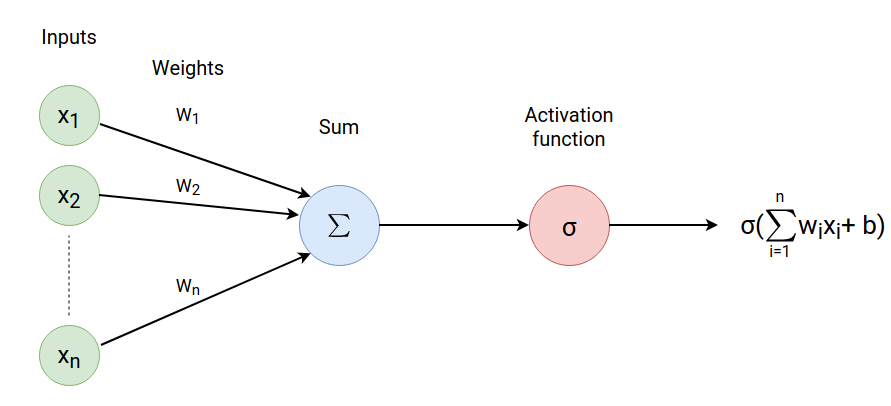
\includegraphics[width=0.9\textwidth]{figures/perceptron.png}
    \caption{The Perceptron}
\end{figure}


The perceptron can model a function of this form: $\sigma(\sum_i^{n} \mathbf{w_i} x_i +b) = \sigma(\mathbf{w}^\top x + b)$. Typical $\sigma$ can be: \\
sigmoid: \ $\frac{1}{1+e^{-x}}$ \quad \quad \quad
tanh: \ $\frac{e^{2x}-1}{e^{2x}+1}$ \quad \quad \quad
ReLU: \ $max(0, x)$ \quad \quad $\cdots$

Notably, the Perceptron is a linear classifier, and as such it famously can't model an XOR \cite{Minskyetal1969}. \\

\begin{figure}[H]
    \centering
    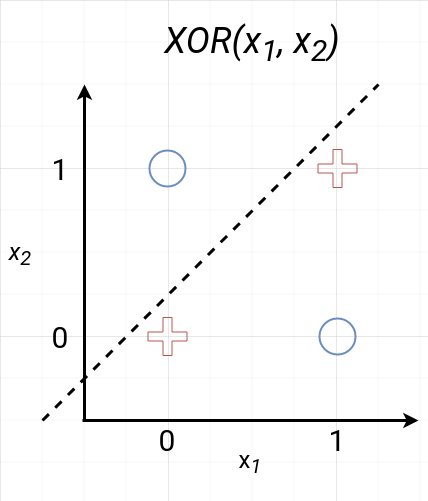
\includegraphics[width=0.35\textwidth]{figures/xor_non_linsep.png}
    \caption{XOR is not linearly separable}
\end{figure}

\subsection{Capacity of multiple neurons}
By allowing ourselves more than 1 neuron in the hidden layer, we can model a XOR and in fact, we get the simplest \textbf{universal approximator}.

\begin{figure}[H]
    \centering
    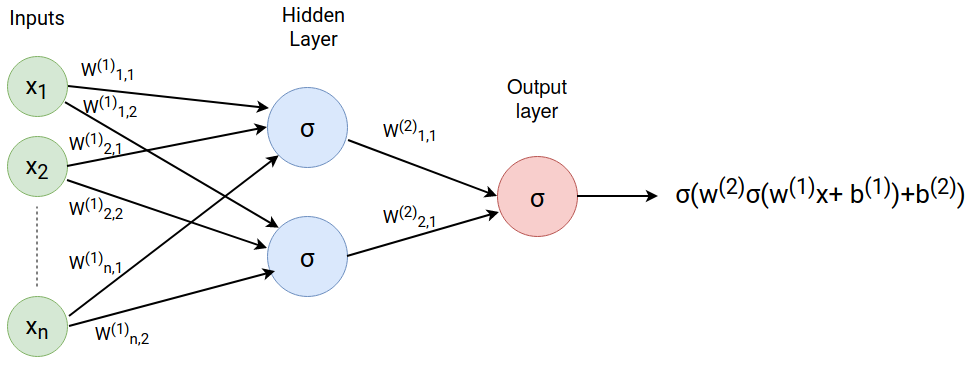
\includegraphics[width=.8\textwidth]{figures/nn.png}
    \caption{A NN with 2 hidden units}
\end{figure}


\section{Universal Approximation Theorem}

The universal approximation theorem states that any continuous function $f :[0,1]^n \xrightarrow{} [0,1]$
can be approximated arbitrarily well by a neural network with at least 1 hidden layer with a finite number of weights, which is what we are going to illustrate in the next subsections. \par

\subsection{Visual proof of Universal Approximation}
In this section we will present a good intuition for the universal approximation theorem by making a summary of this page \href{http://neuralnetworksanddeeplearning.com/chap4.html}{\underline{http://neuralnetworksanddeeplearning.com/chap4.html}}. (All credit is due to \href{http://neuralnetworksanddeeplearning.com/}{\underline{Michael A. Nielsen}} for all the pictures in this subsection) \\

Say we want to approximate a function with 1 input and 1 output like so:
\begin{figure}[H]
    \centering
    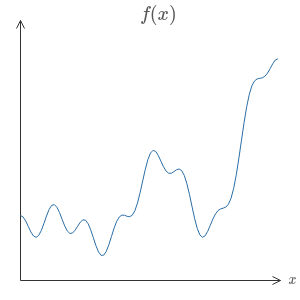
\includegraphics[width=.4\textwidth]{figures/function.png}
    \caption{A continuous function}
\end{figure}

We will first consider a simple NN with 2 hidden neurons that have a sigmoid activation function, and for now the output neuron will just be linear. \\

\textbf{Step 1} Make a step function with 1 of the neuron.
\begin{figure}[H]
    \centering
    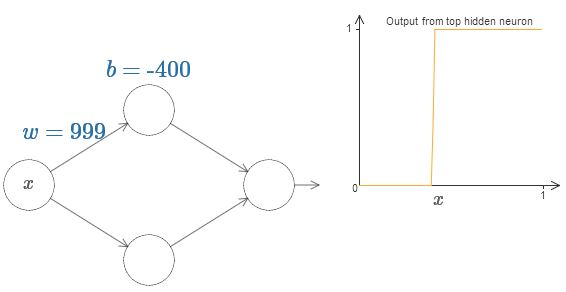
\includegraphics[width=.6\textwidth]{figures/high_weight_function.jpg}
    \caption{Making a step function with the top neuron}
\end{figure}
Let's focus on the top hidden neuron first, by using a big weight on the top neuron we can approximate the step function with a sigmoid arbitrarily well, and by adjusting the bias we can place it anywhere. \\
(Sidenote: the same argument can be made for the tanh activation, but not for ReLu) \\
In this toy example, we won't be interested in changing the weights of the first layer, they just have to be high enough, so we will just consider them to be constant. \\
Additionnaly, to make the plots clearer, we will display the position of the step instead of the bias, which is easily computed with $s = -\frac{b}{w}$. \\
With these changes, the plot above becomes:
\begin{figure}[H]
    \centering
    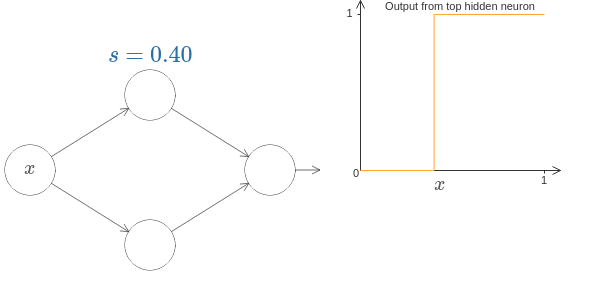
\includegraphics[width=.6\textwidth]{figures/2nn_s.png}
    \caption{Making a step function with the top neuron}
\end{figure}

\textbf{Step 2} Make a "bin" with an opposite step function.
\begin{figure}[H]
    \centering
    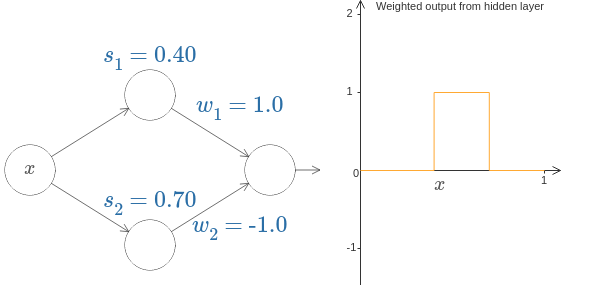
\includegraphics[width=.6\textwidth]{figures/bin.png}
    \caption{Making a bin with 2 opposite step functions}
\end{figure}
As illustrated above, by using the other neuron to make a step function, and setting opposing weights in the second layer, we can effectively approximate a bin and control its position, size and height. \\
Now you can probably see where this is going, to make things even clearer, we will just use 1 value for both $w_1$ and $-w_2$, called $h$, representing the height of the "bin".
\begin{figure}[H]
    \centering
    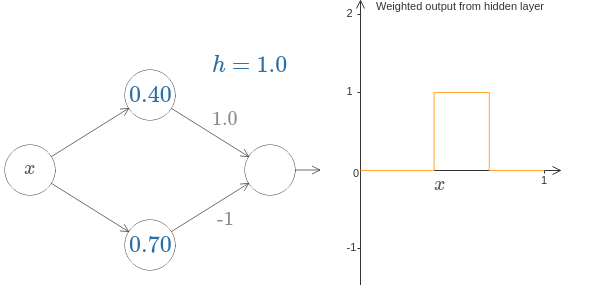
\includegraphics[width=.6\textwidth]{figures/bin_h.png}
    \caption{Making a bin with 2 opposite step functions}
\end{figure}

\textbf{Step 3} Discretize the function.
\begin{figure}[H]
    \centering
    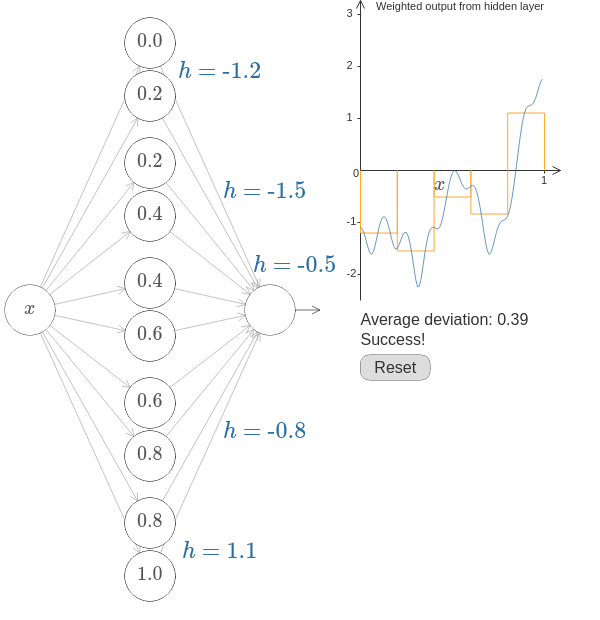
\includegraphics[width=.6\textwidth]{figures/discretize.png}
    \caption{Approximating $f$ with an histogram}
\end{figure}
In this final step, we combine several "bins" to make an histogram approximating the function. Illustrated above is a very rough approximation using only 5 bins (10 hidden units), but we can obviously make it sharper by simply adding more bins. \\\\
$\rightarrow$ Exercise for the reader: if we wanted to use this technique to approximate an \textit{L-Lipschitz} function $f: \mathbb{R} \rightarrow \mathbb{R}$ on the interval $[0, 1]$ with an error at most $\epsilon$ at any point, how many bins would we need ?  

\paragraph{what if i don't want linear neurons in the output layer ?}
The above network's output layer is linear, giving us the histogram approximating $f$, if we add a sigmoid activation function on the output  we just have to approximate $\sigma^{-1}\circ f$ instead of $f$, which we can do with the same method.

\subsection{Cybenko Approximation by Superposition of Sigmoidal Function}
In this subsection we will present the first proven result for Universal Approximation limited to sigmoidal functions, by Cybenko \cite{cybenko1989approximation}. \\
We first define a \textit{sigmoidal function} $\sigma$ as:
$$
\sigma(x) \to
\begin{cases}
1 \text{\quad as } x\to+\infty \\
0 \text{\quad as } x\to-\infty
\end{cases}
$$
\textit{Note: while sigmoidal functions are usually assumed to be monotonic increasing, this assumption is not necessary for this result.}

\begin{thm}
Let $C([0,1]^n)$ denote the set of all continous function $[0, 1]^n \to \mathbb{R}$, let $\sigma$ be any sigmoidal activation function then the finite sum of the form   
$f(x) = \sum_{i=1}^{N} \alpha_i \sigma(\mathbf{w_i}^\top x +b_i)$ is dense in $C([0,1]^n)$
\end{thm}

Informaly, this theorem is saying that for any $g \subset C([0,1]^n)$ and any $\epsilon >0$, there exists $f: x \rightarrow \sum_{i=1}^{N} \alpha_i \sigma(\mathbf{w_i}^\top x +b)$ such that $|f(x)-g(x)|<\epsilon$ for all $x \subset [0,1]^n$.
\[
\begin{tikzpicture}
  \begin{axis}[ 
    xlabel=$x$,
    ylabel=$y$,
    width=10cm
  ] 
    \addplot[black ] {sin(deg(x))};
    \addplot[red,dashed ] {sin(deg(x))+sin(deg(x*10))*0.2};
     \node[below,black] at (450,0.8) {absolute difference between $f(x)$ and $g(x)$ is $\epsilon$};
    \legend{$f(x)$, $g(x)$}
  \end{axis}
\end{tikzpicture}
\]
A similar result was independently obtained by Hornik\cite{hornik1989multilayer} and also by Funahashi\cite{funahashi1989approximate} using different tools. Hornik's proof relies on the Stone-Weierstrass Theorem which states that every continuous function defined on a closed interval $[a, b]$ can be uniformly approximated as closely as desired by a polynomial function.

\subsection{Kolmogorov-Arnold Representation theorem}
The Kolmogorov-Arnold representation theorem (or superposition theorem) \cite{kolmogorov1957representation} states that every multivariate continuous function can be represented as a superposition of continuous functions of one variable.\par
It solved a more general form of Hilbert's thirteenth problem \cite{abhyankar1997hilbert} which was questioning whether a solution to $7^{th}$ degree equations could be expressed by a finite sum of two-variable functions.\par

\begin{thm}
Any continuous function $f :[0,1]^n \xrightarrow{} \mathbb{R}$ can be written as 
$$ f(x) =f(x_1,..,..,x_n) =  \sum_{q=1}^{Z_m} \phi_q\left(\sum_{q=1}^{m} \Psi_q(x_q)\right) $$
\end{thm}
This implies, among other things, that if we could chose the non-linearity of each unit we can represent any continuous function \textbf{exactly} with a NN with 1 hidden layer.


\section{The expressive power of Deep neural networks}

\subsection{A view from the width (Lu et al. 2017)}
In the previous sections, we focused on the setting of depth-bounded (e.g. depth-2) neural networks. With \cite{lu2017expressive} we're going to see some interesting results for \textbf{width-bounded} neural networks instead !

\begin{thm}
(Universal Approximation Theorem for Width-Bounded ReLU Networks).
For any Lebesgue-integrable function $f:\mathbb{R}^n \to \mathbb{R}$ and any $\epsilon > 0$, there exists a fully-connected ReLU network $A$ with width $d_m \leq n + 4$, such that the function $F_A$ represented by this network satisfies
$$\int_{\mathbb{R}^n} |f(x)-F_A(x)|dx < \epsilon$$
\end{thm}
This theorem states that any continuous function $f: \mathbb{R}^n \to \mathbb{R}$ can be approximated by a deep ReLU network with width $\leq n+4$.

\begin{thm}
    Let $n$ be the input dimension. For any integer $k \geq n+4$ there exists $F_{\alpha}: \mathbf{R^n} \rightarrow \mathbf{R}$ represented by a relu neural network $\alpha$ with width $d_m= 2k^2$ and depth $h=3$ such that for any constant $b>0$, there exists an $\epsilon>0$ and for any function $F_{\beta}: \mathbf{R^n} \rightarrow \mathbf{R}$ represented by a ReLu neural network $\beta$ whose parameters are bounded in $[-b,b]$ with width $d_m \leq k^{\frac{3}{2}}$ and depth $h \leq k+2$ the following inequality holds
    $$\int_{\mathbf{R}} |F_{\alpha} - F_{\beta}| dx \geq \epsilon$$
\end{thm}

This theorem states that there are networks such that reducing width requires increasing in the size to compensate, which is similar to that of depth qualitatively.

\subsection{Representation benefits of deep NN (Telgarsky 2015)}
In this section, we want to show interesting results from \cite{telgarsky2015representation}, that will allow us to compare the expressivity of wide networks against deep and recurrent networks, on a specific classification problem defined below: \\

Let n-ap (\textit{n-alternating-points}) be the set of $n := 2^k$ points  uniformly spaced within $[0, 1-2^{-k}]$ with alternating labels.
\begin{figure}[H]
    \centering
    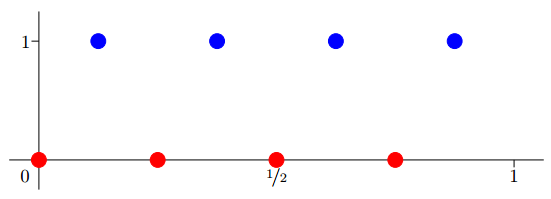
\includegraphics[width=.6\textwidth]{figures/nap.png}
    \caption{The $2^3$-ap \cite{telgarsky2015representation}}
\end{figure}

In the following theorems we will note $\mathscr{N}(\sigma, l, m)$ the set of function given by a feedforward neural network with activation $\sigma$ and $l$ layers with at most $m$ nodes. The ReLU activation will be noted $\sigma_R$ and the classification error $\mathcal{R}_z$.

\begin{thm}
With $m \leq 2^{(k-3)/(l-1)}$, for any positive integer $k$, $\exists$ a collection of $n:=2^k$ points $S = (x_i,y_i)^n_{i=1}$ where $x_i \in [0, 1], y \in \{0, 1\}$ such that \\
$$\min_{f\in\mathscr{N}(\sigma_R, m, l)} \mathcal{R}_z(f) = \frac{1}{6} \quad \quad \text{and} \quad \quad \min_{g\in\mathscr{N}(\sigma_R, 2, 2k)} \mathcal{R}_z(g) = 0$$
\end{thm}

Notably, if we look at the case of 2 layered networks, this tells us that even with $2^{k-3}$ units in the hidden layer, the wide network is going to missclassify $\frac{1}{6}$ of the points, whereas a deep network with $2k$ hidden layers with 2 units each can achieve 0 classification error. \\\\

Now we will refine this result, let $\mathscr{R}(\sigma, l, m, k)$ denote k iterations of a recurrent neural network, every $f \in \mathscr{R}(\sigma, l, m, k)$ can be expressed as some fixed network $g \in \mathscr{N}(\sigma, l, m)$ applied k times:
$$f(x) = g^k(x) = \underbrace{(g\circ g \cdots \circ g)}_\text{k times}(x)$$

Consequently, $\mathscr{R}(\sigma, l, m, k) \subseteq \mathscr{N}(\sigma, l, mk)$ but the former has $\mathcal{O}(ml)$ parameters whereas the latter has $\mathcal{O}(mlk)$ parameters. \\
Lastly we define the following functions:

\begin{defn}[Sawtooth]
A function $f: \reals \xrightarrow{} \reals$ is $t$-sawtooth if it is piece-wise linear with $t$-pieces
\end{defn}
We can say for example that $\sigma_R$ (ReLU) is a 2-sawtooth function, decision stumps used in boosting are also 2-sawtooth, and decision trees with t-1 nodes are t-sawtooth.

\begin{thm}
Let positive integer k, number of layers l, and number of nodes per layer $m$ be given. \\
Given a t-sawtooth $\sigma : \mathbb{R} \to \mathbb{R}$ and $n := 2k$ points as specified by the n-ap, then \\
$$\min_{f\in\mathscr{N}(\sigma, m, l)} \mathcal{R}_z(f) \geq \frac{n-4(tm)^l}{3n} \quad \quad \text{and} \quad \quad \min_{g\in\mathscr{R}(\sigma_R, 2, 2, k)} \mathcal{R}_z(g) = 0$$
\end{thm}
In summary, this means that on the $2^k$-ap, one needs exponentially (in k) many parameters with a wide network, linearly many parameters with a deep network and constantly many parameters with a recurrent network.

\subsubsection{Upper bound proof [WIP]}
\begin{lemma}
If f is t-sawtooth, g is s-sawtooth, then we have \\
$f+g$\ \ is (s+t)-sawtooth \quad \quad \quad $f\circ g$\ \ is st-sawtooth
\end{lemma}
\begin{lemma}
If $\sigma$ is t-sawtooth, then every f \in \mathscr{N}($\sigma$;m,l) is $(tm)^l$-sawtooth
\end{lemma}

Let us define the "mirror map" $f^k_m: \mathbb{R}\to\mathbb{R}$ as figure shows:
\begin{figure}[H]
    \centering
    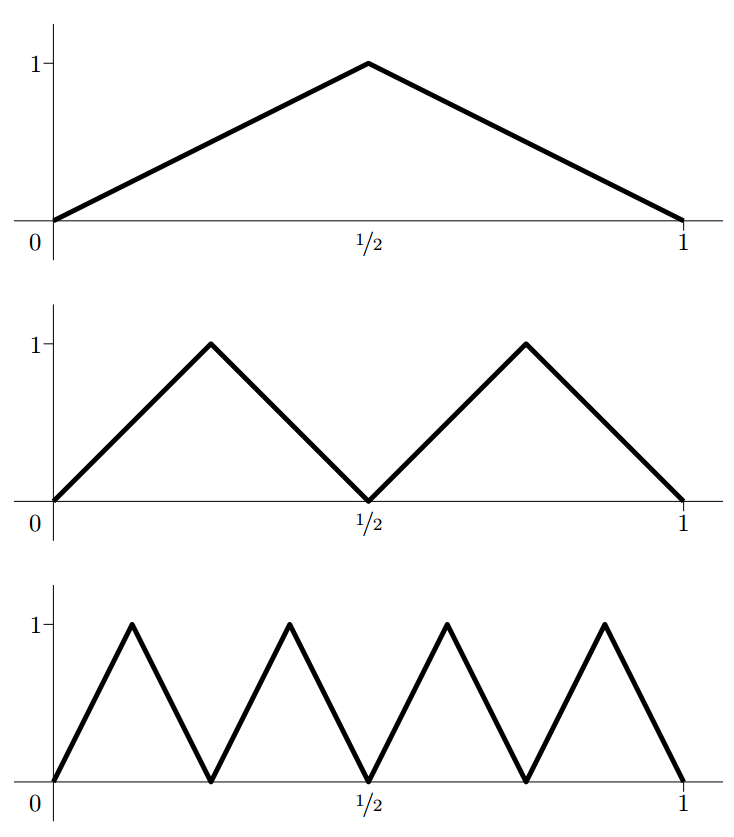
\includegraphics[width=.6\textwidth]{figures/fmk.png}
    \caption{$f_m$, $f^2_m$ and $f^3_m$ \cite{telgarsky2015representation}}
\end{figure}

Note that $f^k_m \in \mathscr{R}(\sigma_R;2,2,k) \subseteq \mathscr{N}(\sigma_R;2,2k)$.

%----------------------------------------https://www.overleaf.com/project/5c6c50cc5b86f10a80c2eff0
% \section*{Acknowledgments} 

%----------------------------------------
\bibliographystyle{abbrvnat}
\bibliography{Refs/lec11}
%----------------------------------------

\end{document}
 